\chapter{Likelihood ratio tests and profile likelihood}
\subsection{Likelihood ratio test} 
The parameter estimation is done with  a maximum likelihood method, 
this gives the 
opportunity to easily test different hypotheses against others, when the hypotheses are hierarchical (e.g. Casella and Berger 1996). For example,
we wish to test if the migration rates are the same 
in a two population model with 4 parameters: 
\begin{align}
H_0:& \M_{21} = \M_{12}\qquad \Theta_1 = {\hat \Theta_1},\Theta_2 = {\hat \Theta_2},\\
H_1:& \M_{21} \neq \M_{12}\qquad \Theta_1 = {\hat \Theta_1},\Theta_2 = {\hat \Theta_2},\\
\intertext{and then can test using the test statistics}
-2& \log\left(\frac{{\rm L}(\Theta_x)}{{\rm L}(\hat\Theta)}\right) \le \chi^2_{df,\alpha}\label{LRATIOFORM}
\end{align}
In the example the degrees of freedom would be two: we are 
changing two parameters.
We need to run {\tt migrate} with the full model: all parameter can vary
independently. We get parameter estimates ${\hat \Theta_1}$, ${\hat \Theta_2}$,
${\hat \M_{21}}$, and ${\hat \M_{12}}$. We compare this maximum likelihood
with the likelihood when we restrict the migration rate to be the same
for example the mean of both estimates. The ratio between these two likelihoods
is in the limit (if there is a huge amount of data) $\chi^2$ distributed 
(Formula \ref{LRATIOFORM}, Figure \ref{LRATIOFIG}). 
If the probability is smaller than $0.05$ we would reject the 
Null-hypothesis and accept the alternative, saying that the values
are not equal.
If you have mtDNA data this methods is theoretically not applicable, because
you cannot increase the data beyond the full sequence of the mitochondrion,
but I am pretty sure that for most situations the test will 
still work. 
There is a problem due to the implementation of the program that we can
not allow that parameters go to 0.0. A parameter of 0.0 has a 0.0 probability. 
we would need to correct for the fact that our parameter might be on the boundary of its range.
If we assume that the parameters are independent then under some conditions we can calculate 
a test statistic that takes this boundary condition into account [but this is not yet yet implemented in the
l-ratio test]. If you test just if a single parameter is 0.0 then the test needs a halved significance level (cit).
\begin{figure}[htb]
\begin{center}
\leavevmode
\hbox{%
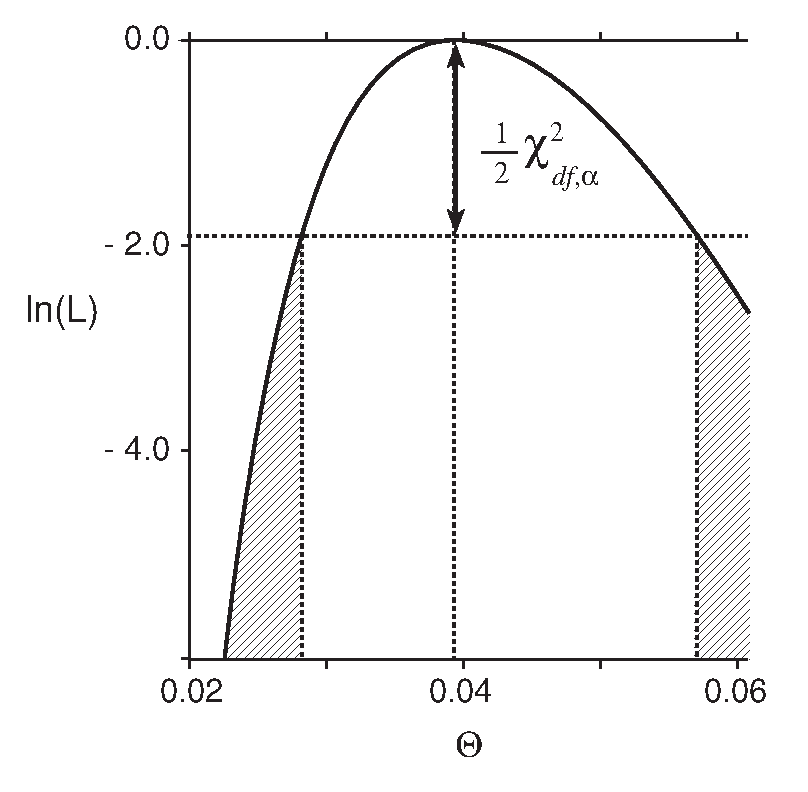
\includegraphics[scale=0.6]{mim/coalesce_likecurve}}
\end{center}
\caption{Likelihood ratio test: dashed areas are outside of the 95\% confidence limit. $\Theta$ is $4 N_e \mu$; $df=1$, $\alpha=0.05$ \label{LRATIOFIG}}
\end{figure}

Do not forget that these likelihoods are only 
approximations. Comparison with exact likelihoods for
genealogies with 3 tips and no migration show that the MCMC curves are
exactly the same as the ``exact'' curves. When the program is not run long 
enough the MCMC curves tend to be wider than the ``exact'' curves and 
have their maximum biased towards the parameter value at which we run the chains. We expect
when there are many sampled individuals that it is likely that you
run the program not long enough and therefore will get wrong confidence
interval estimates and will stick too close to the start parameters.
(Figure \ref{EXACT_MCMC}). 
You can check for this by running the program several
times from very different start values. Just looking at the point estimates
is probably not enough, you should to inspect the profile likelihoods, too.
Most of the time it seems that real single locus data is not very great for
the estimation of migration rates and the ``confidence'' intervals are huge. 
\begin{figure}[htb]
\begin{center}
\leavevmode
\hbox{%

\includegraphics[scale=0.6]{mim/exact_and_mcmc}}
\end{center}
\caption{Log likelihood curves from (a) the exact likelihood 
calculation for a genealogy with 3 samples, (b) an MCMC based estimator
with only one (1) sampled genealogy with start value $\Theta_0=\text{Watterson estimate}$, 
(c) with one acceptance using a $\Theta_0=0.00001$. The data are 3 sequences each
1000 bp long and generated with a $\Theta=0.1$, running the program some 1000
genealogies delivers a likelihood curve indistinguishable from the exact likelihood curve.
\label{EXACT_MCMC}}
\end{figure}

For the {\tt parmfile} there is an option {\bt{l-ratio}} which you can use to 
define a hypothesis against the program run (Null-hypothesis). 
You can repeat the statement for testing more than one hypothesis,
but you may need to correct your significance level for multiple tests. 
The syntax is:\\
{\bt{l-ratio:$<$YES$>$ $<$:param1,param2,param3,....paramn*n$>$}}\\
\begin{description}
\item{\bt{Means}} over all loci
\end{description}
The syntax for each {\bt{param1, param2,...}} is rather complicated:
{\bt{param1 = $<$* $|$x $|$  m $|$ value$>$}}\\
\begin{description}
\item{\bt{*}} the value is the same as the one from the estimate ($=H_1$)
\item{\bt{x}} the value will be maximized.
\item{\bt{m}} the value is the mean of the parameters, either $\Theta$ or $\M$.
\item{\bt{s}} the parameters is symmetric in $\M$.
\item{\bt{S}} the parameter is symmetric in $\Theta\M= hN_em$ (h is the inheritance factor: 4 for diploids, 2 for haploids, 1 for haploids passed on by one sex).
\item{\bt{value}} is any arbitrary value you want to test.
\end{description}
Examples for two populations for the parmfile entries:\\
{\bt{l-ration=YES:0.01,1.0,1.1,0.011;\\
l-ratio=YES:*,m,m,*;\\
l-ratio=YES:x,1.34,*,0;
}}
\smallskip%\multicolumn{1}{c}{
For the test you need to to specify the migration matrix with $\Theta$ values on the diagonal.
The parameters are ordered like this:\\
\begin{tabular}{ccccc}
$\Theta_1$, & $\M_{2,1}$,& $\M_{3,1}$,& ...,& $\M_{n,1}$,\\
$\M_{1,2}$,& $\Theta_2$,&  $\M_{3,2}$,& ...,& $\M_{n,2}$, \\
\multicolumn{5}{c}{...}\\
\multicolumn{3}{c}{...}& $\M_{(n-1),n}$,& $\Theta_n$
\end{tabular}

The calculations are always done using the scaled migration rate $\M$ but are adjusted according to the options and might print out hNm.\medskip
Example with 3 populations based on the following migration matrix:
\begin{gather}
\begin{matrix}
- &2&1\\
1.8&-&1\\
0.5&0.6&-
\end{matrix} \nonumber
\end{gather}
results in the string\\
{\bt{l-ratio=YES:*, 2,1,1.8,*,1,0.5,0.6,*;}}

Do not forget the semicolon at the end [ a comma will do too, but NO comma or semi-colon might fail].
\newpage
\section{Profile likelihood}
Parameter estimation in high dimensions causes serious problems 
in the presentation of results: for 2 population we have 4 parameters,
with 8 population 64, etc. One would like to show the high dimensional surface
but we are crudely limited to 3 and perhaps can understand graphs up to five.
Showing one parameter at a time only shows us a transection through the solution space, but is perhaps the best we can do. By using profile likelihoods
we can trace a parameter and also see how the other parameter change at given 
values for our profile parameter. Instead of finding the parameters at the maximum likelihood, we fix the profile parameter at some arbitrary value and then maximize the other parameters at that profile likelihood. This constructs a path through the solution space, which we can use to construct approximate confidence limits
using the likelihood ratio test criteria (Fig \ref{PROFILEFIG}) with a degree of freedom of 1 (well, this is true in ``asymptopia'' 
but may produce very tight confidence intervals \cite{beerli:2001:mle}. Several advanced statistic textbooks discuss the use of likelihood ratio and
the related profile likelihoods \cite[e.g. ][]{casella:1996}, but I like the compact,
and in my opinion, very readable, short text of \cite{meeker:1995:taa}. 
 
\begin{figure}[htb]
\begin{center}
\leavevmode
\hbox{%
\includegraphics[scale=0.6]{mim/profile_real}}% profile.example
\end{center}
\caption{{Profile likelihood, for a series of values of a parameter, the other parameter are maximized and the likelihood given that parameter is highest along the straight lines in A. (A) Contour plots for a run with two variables,
the thick lines are the 50\%, 95\%, and 99\% confidence contours. (B) is the
profile likelihood curve for $\Theta$ and (C) is the profile likelihood curve
for 4Nm (based on $\M$). The 95\% confidence range for B and C are for values 
with log likelihood values above -2.} 
\label{PROFILEFIG}}
\end{figure}

%\caption{Profile likelihood, for a series of values of a parameter, the other parameter are maximized and the likelihood given that parameter is highest along the thick line. The contours are approximate confidence areas based on the likelihood ratio test. The star is the maximum likelihood estimate for all
%parameters}
\newpage